% Midterm Report

% Your milestone report should be 1 - 2 (max) pages and answer the following questions:
% 1. What has been done so far? (tools decided on, implementations, overview on methods, …)
% 2. First Results (e.g., some raw plots)
% (no explicit introduction, because you described your topic already in the proposal)

% The milestone report must report on at least one experiment that you have done since the proposal. This experiment does not need to be successful, but you should have attempted something. If it did not work as expected, you should briefly discuss why. You are encouraged to include a plot or figure.

% The format for the report has to be the standard IEEE conference format: https://www.ieee.org/conferences/publishing/templates.html

\documentclass[conference]{IEEEtran}
\usepackage{cite}
\usepackage{amsmath,amssymb,amsfonts}
\usepackage{algorithmic}
\usepackage{graphicx}
\usepackage{textcomp}
\usepackage{xcolor}
\ifCLASSOPTIONcompsoc
\usepackage[caption=false,font=normalsize,labelfon
t=sf,textfont=sf]{subfig}
\else
\usepackage[caption=false,font=footnotesize]{subfi
g}
\fi
\def\BibTeX{{\rm B\kern-.05em{\sc i\kern-.025em b}\kern-.08em
    T\kern-.1667em\lower.7ex\hbox{E}\kern-.125emX}}

\begin{document}


\title{Milestone Report}

\author{\IEEEauthorblockN{Franziska Schwaiger}
    \IEEEauthorblockA{\textit{Matriculation number: 03658670}}
    \and
    \IEEEauthorblockN{Thomas Brunner}
    \IEEEauthorblockA{\textit{Matriculation number: 03675118}}
}

\maketitle

\section*{Dataset}

\begin{figure*}[t]
    \centering
    \subfloat[2 DOF]{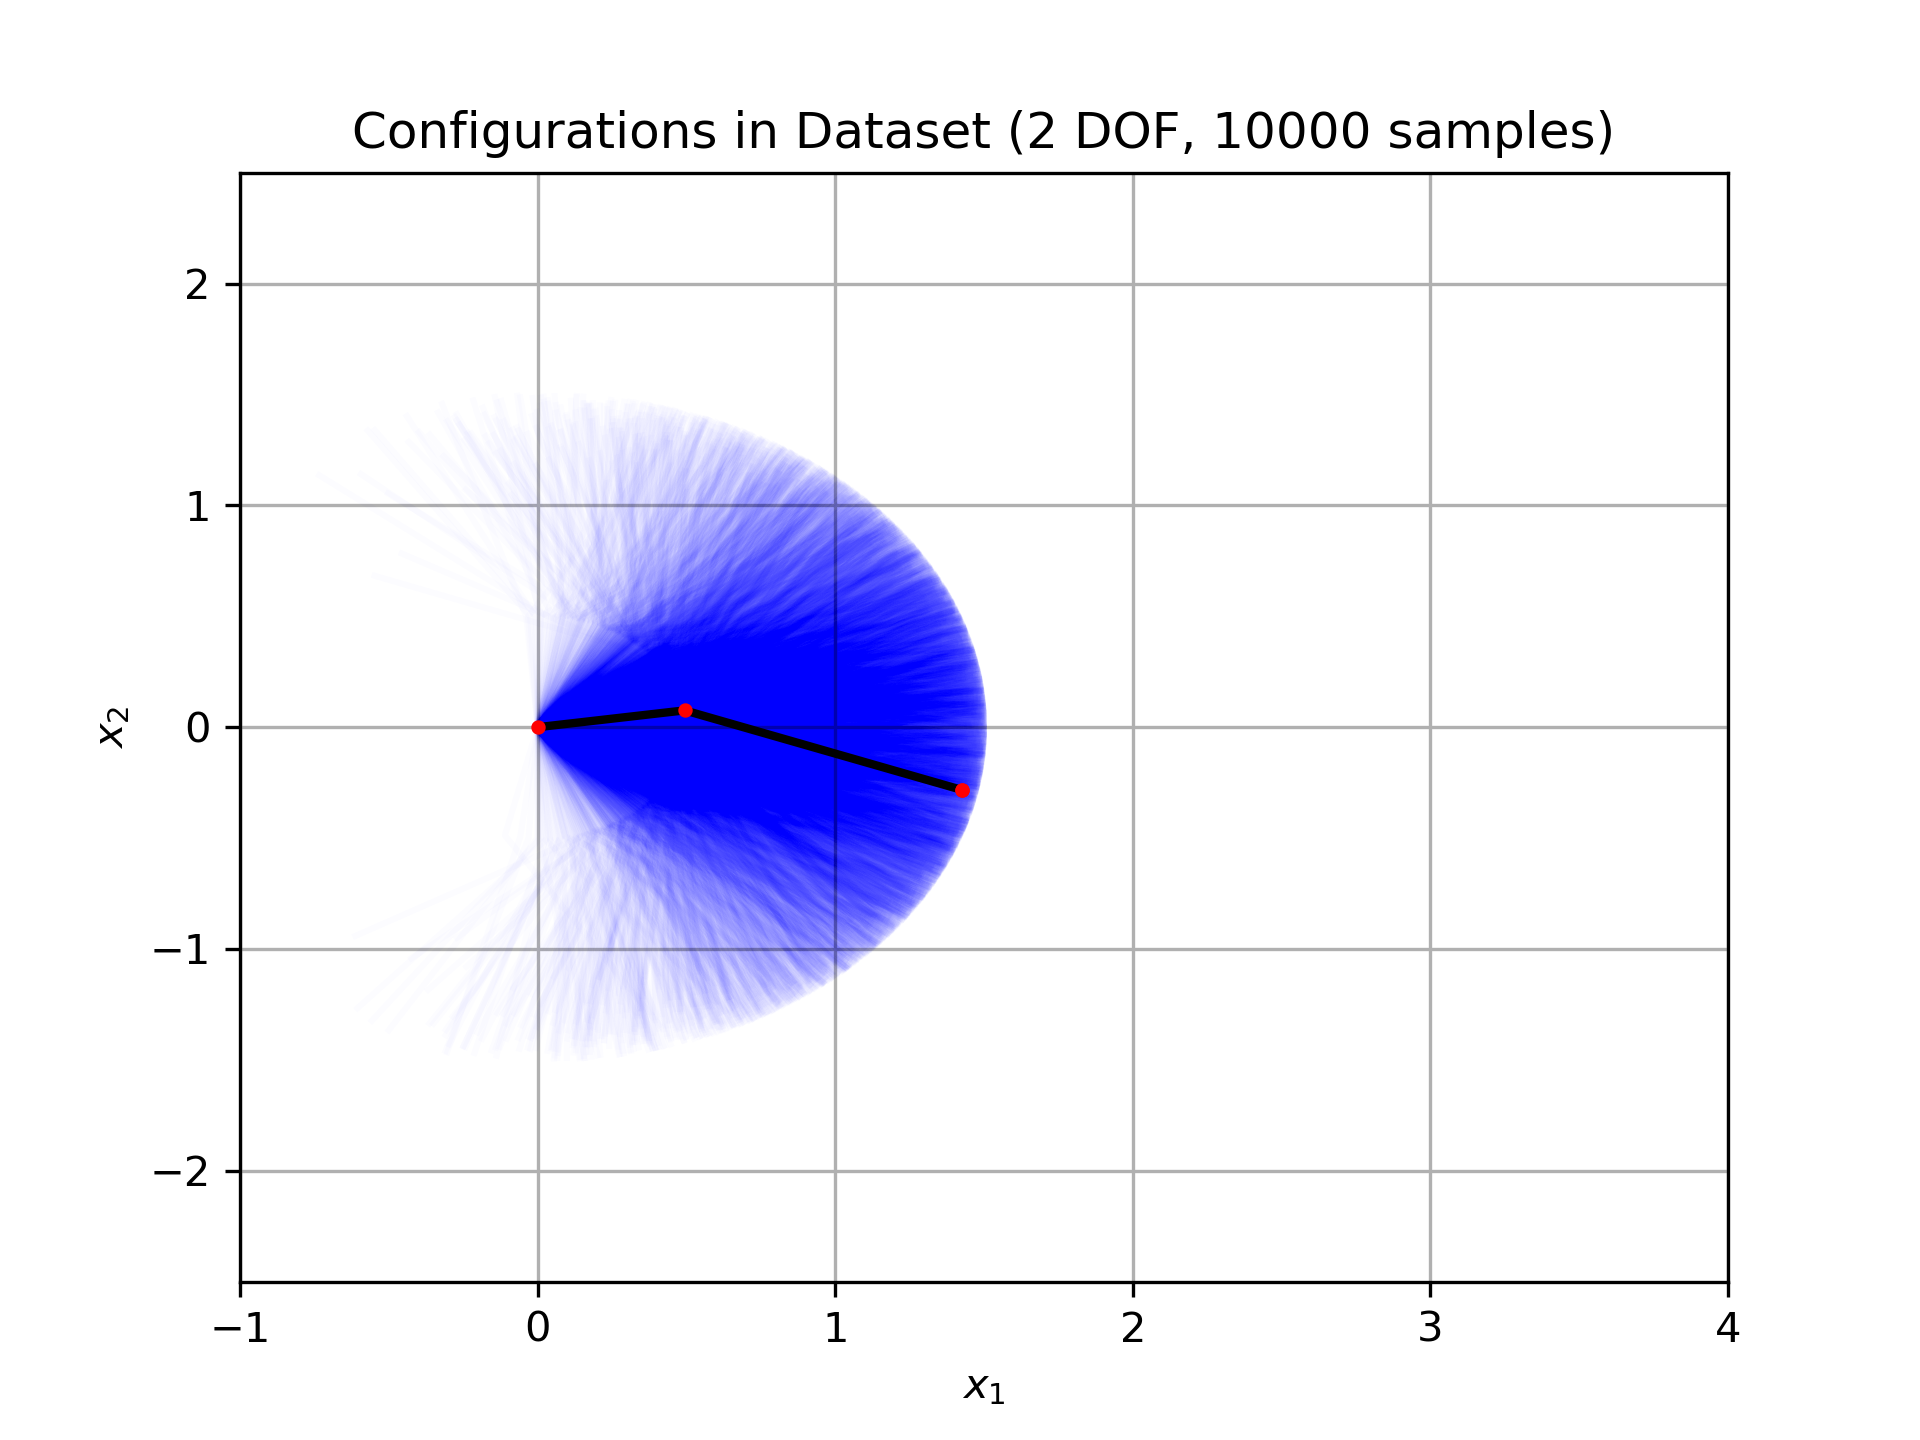
\includegraphics[width=0.3\linewidth]{figures/normal_2dof_configs.png}
        \label{fig_first_case}}
    \subfloat[3 DOF]{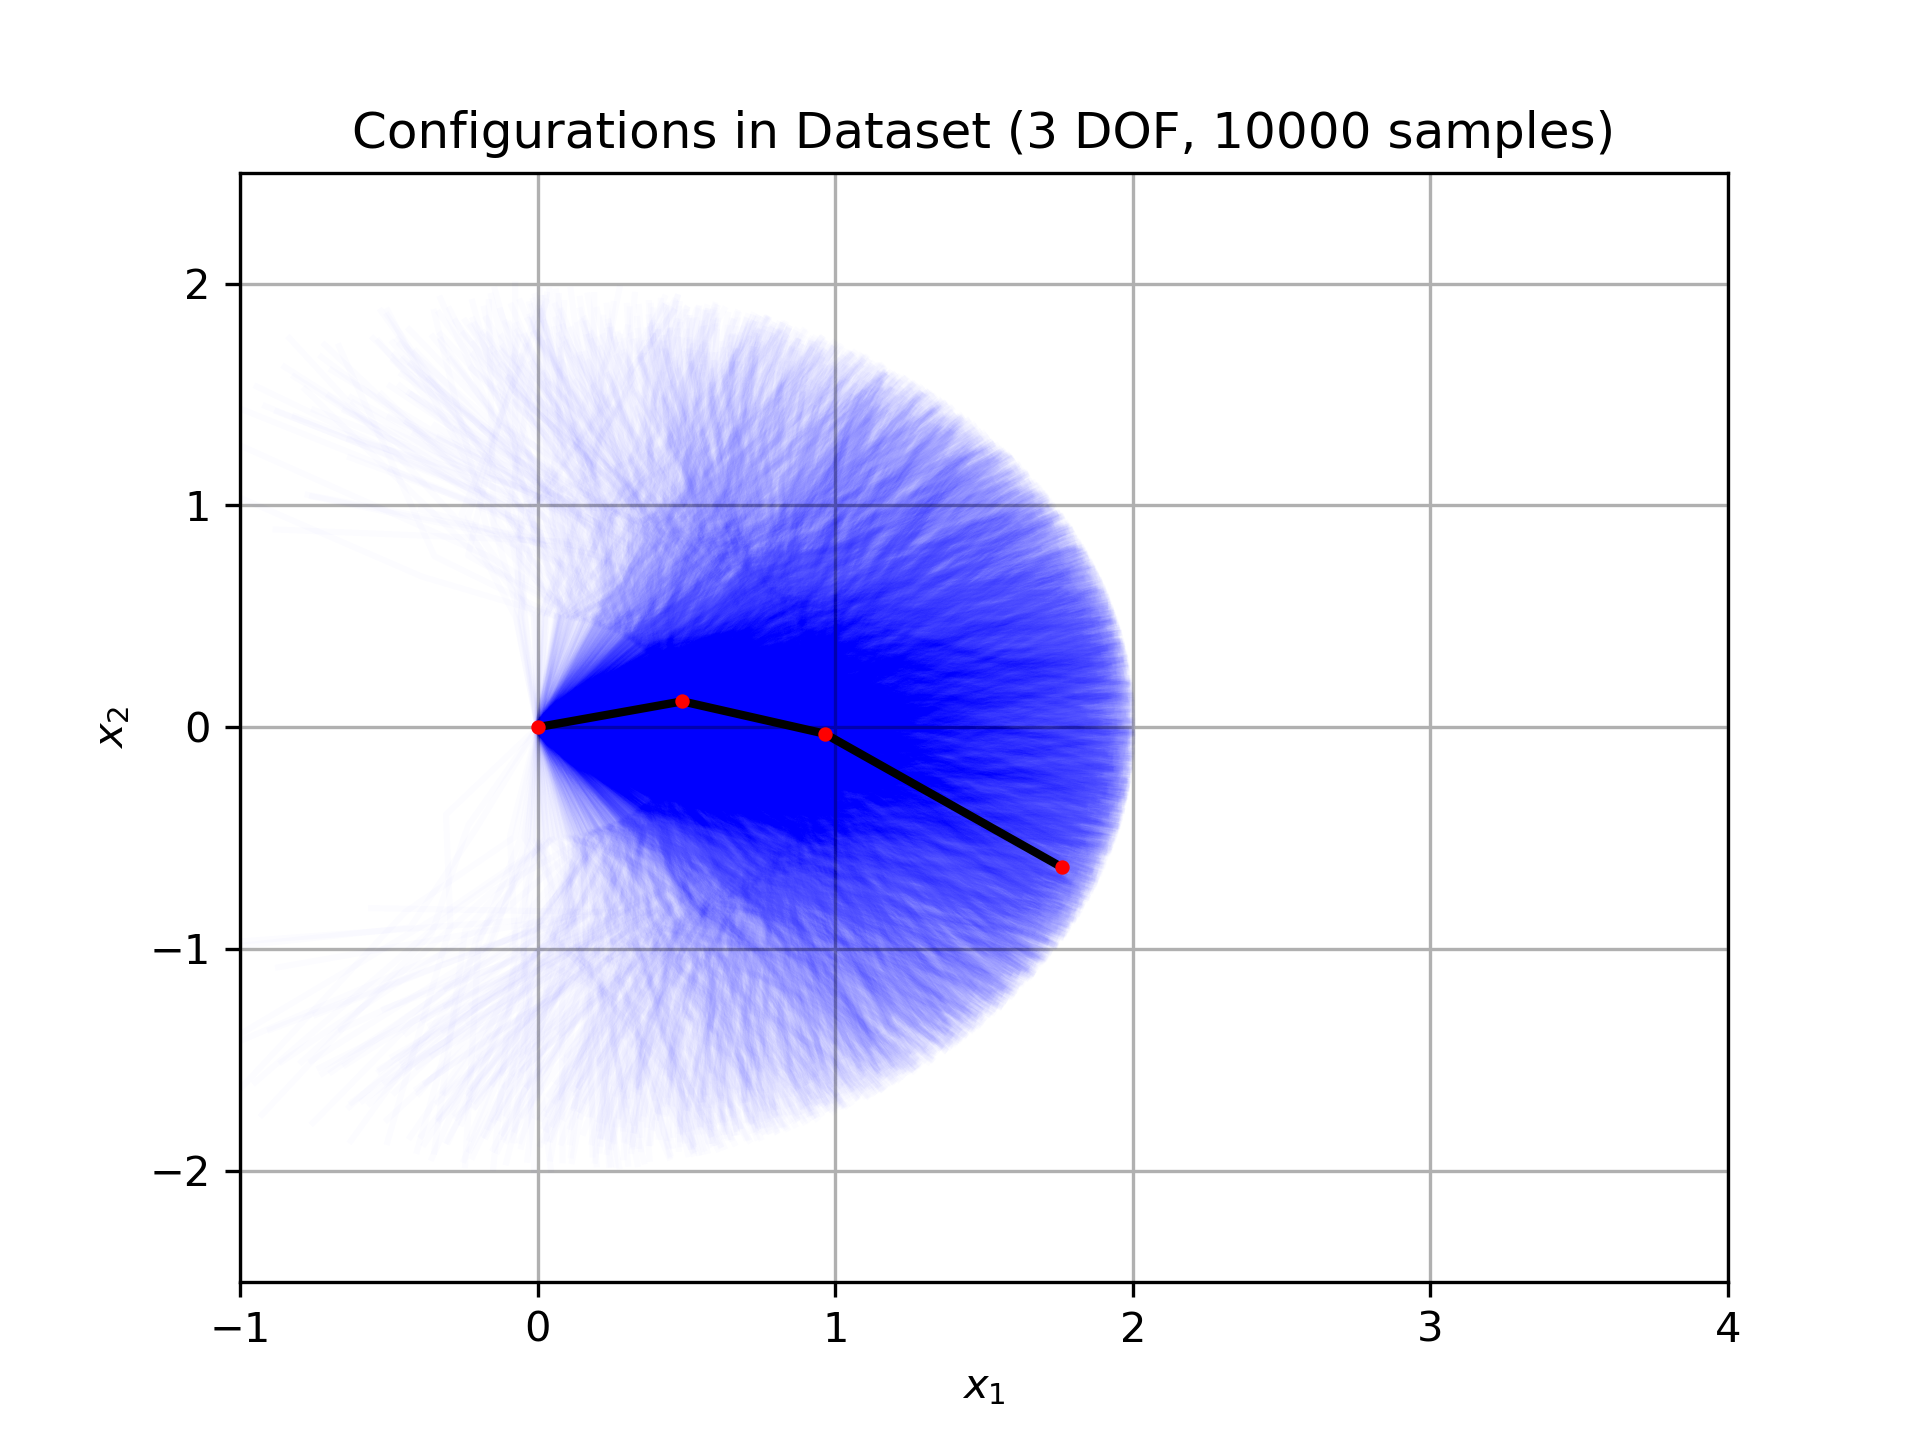
\includegraphics[width=0.3\linewidth]{figures/normal_3dof_configs.png}
        \label{fig_second_case}}
    \subfloat[4 DOF]{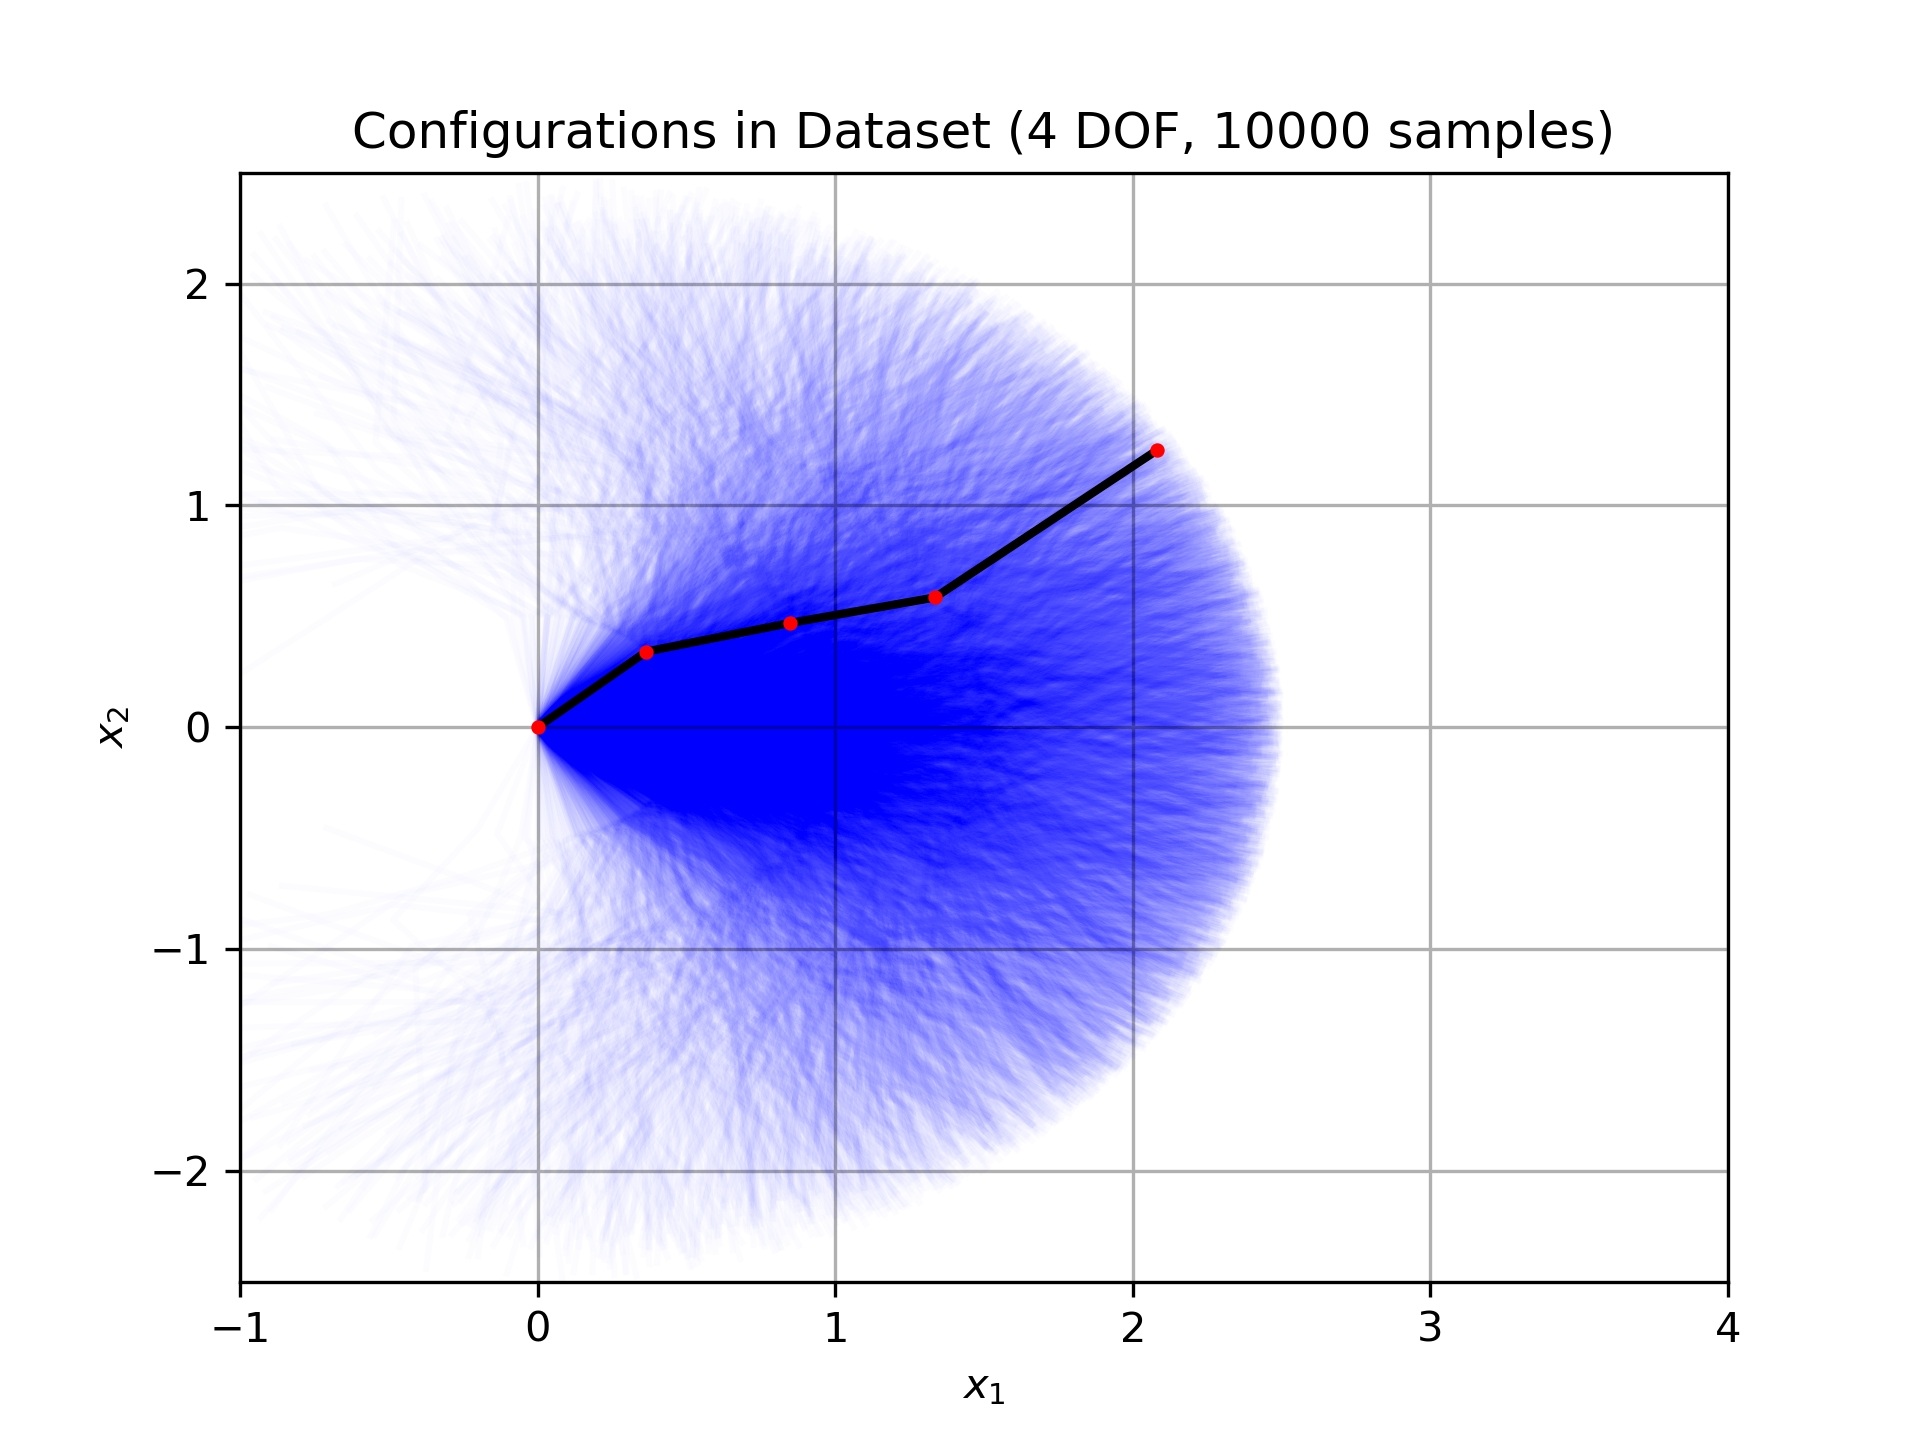
\includegraphics[width=0.3\linewidth]{figures/normal_4dof_configs.png}
        \label{fig_second_case}}
    \caption{Illustration of datasets used during training of models. Only a subset of the samples contained in the datasets is shown here. One configuration in the dataset is highlighted to illustrate the configuration of the robot arm.}
    \label{fig_sim}
\end{figure*}


\section*{Methods}

\subsection*{Conditional Variational Autoencoder}

\subsection*{Invertible Neural Network}

\section*{Experimental Evaluation}

\subsection*{Evaluation protocol}
\subsection*{Results}


\section*{Next Steps}


\nocite{*}
\bibliographystyle{IEEEtran}
\bibliography{IEEEabrv,midterm_report}

\end{document}
